\documentclass[titlepage, a4paper, 12pt]{article}
\usepackage[swedish]{babel}
\usepackage[utf8]{inputenc}
\usepackage{verbatim}
\usepackage{fancyhdr}
\usepackage{graphicx}
\usepackage{parskip}

% SourceCode
\usepackage{listings}
\usepackage{color}

% Include pdf with multiple pages ex \includepdf[pages=-, nup=2x2]{filename.pdf}
\usepackage[final]{pdfpages}
% Place figures where they should be
\usepackage{float}

% SourceCode
\definecolor{keywordcolor}{rgb}{0.5,0,0.75}
\lstset{
  inputencoding=utf8,
  language=Java,
  extendedchars=true,
  basicstyle=\scriptsize\ttfamily,
  stringstyle=\color{blue},
  commentstyle=\color{red},
  numbers=left,
  firstnumber=auto,
  numberblanklines=true,
  stepnumber=1,
  showstringspaces=false,
  keywordstyle=\color{keywordcolor}
  % identifierstyle=\color{identifiercolor}
}

% Float for text
\floatstyle{ruled}
\newfloat{kod}{H}{lop}
\floatname{kod}{Kodsnutt}

% vars
\def\title{Termiter i NetLogo}
\def\preTitle{Laboration 1}
\def\kurs{Emergenta system, VT-09}

\def\namn{Andreas Jakobsson}
\def\mail{dit06ajs@cs.umu.se}
\def\namnTva{Anton Johansson}
\def\mailTva{dit06ajn@cs.umu.se}

\def\pathtocode{$\sim$dit06ajn/edu/emergenta-system/lab1/src}

\def\handledareEtt{Jonny Pettersson, jonny@cs.umu.se}
\def\handledareTva{Anders Broberg, bopspe@cs.umu.se}

\def\inst{datavetenskap}
\def\dokumentTyp{Laborationsrapport}

\begin{document}
\begin{titlepage}
  \thispagestyle{empty}
  \begin{small}
    \begin{tabular}{@{}p{\textwidth}@{}}
      UMEÅ UNIVERSITET \hfill \today \\
      Institutionen för \inst \\
      \dokumentTyp \\
    \end{tabular}
  \end{small}
  \vspace{10mm}
  \begin{center}
    \LARGE{\preTitle} \\
    \huge{\textbf{\kurs}} \\
    \vspace{10mm}
    \LARGE{\title} \\
    \vspace{15mm}
    \begin{large}
      \namn, \mail \\
      \namnTva, \mailTva\\
      \texttt{\pathtocode}
    \end{large}
    \vfill
    \large{\textbf{Handledare}}\\
    \mbox{\large{\handledareEtt}}
    \mbox{\large{\handledareTva}}
  \end{center}
\end{titlepage}

\newpage
\mbox{}
\vspace{70mm}
\begin{center}
% Dedication goes here
\end{center}
\thispagestyle{empty}
\newpage

\pagestyle{fancy}
\rhead{\today}
\lhead{\footnotesize{\namn, \mail\\\namnTva, \mailTva}}
\chead{}
\lfoot{}
\cfoot{}
\rfoot{}

\cleardoublepage
\newpage
\tableofcontents
\cleardoublepage

% \fancyfoot[LE,RO]{\thepage}
\cfoot{\thepage}
\pagenumbering{arabic}


\section{Inledning}
Denna laboration ska undersöka den emergenta egenskapen som uppstår
med myror som var och en följer följande enkla regler:

\begin{itemize}
 \item Vandra slumpmässigt omkring (utan bärande på träbit)
 \item Vid kontakt med en träbit, plocka upp den
 \item Vandra slumpmässigt omkring (bärande på träbit)
 \item Vid kontakt med en träbit, lägg ned den egna träbiten brevid den nya
 \item Hoppa till första punkten igen
\end{itemize}

Med hjälp av dessa enkla regler kan det i interaktion mellan myror
(eller en myra med sig själv över tid) uppträda den globala egenskapen
av en samlad hög.

\section{Problemspecifikation}\label{sec:problemspecifikation}
Laborationen gick ut på att göra ändringar i en befintlig
NetLogo\footnote{http://ccl.northwestern.edu/netlogo/} modell som
imiterar myrors beteende att bygga myrstackar. Ändringarna som skulle
göras och studeras var:

\begin{itemize}
\item Sortering av flera sorters träbitar för att bygga olika
  myrstackar.
\item Laborera med feltolerans, vad händer med modellen om det införs
  myror som på något sätt stör de andra myrornas beteende?
\end{itemize}
% Behövs det ytterligare regler i termiterna för att systemet ska
% konvergera till en separat hög för varje sorts träbitar?

\subsection{Frågor denna rapport behandlar}
Följande lista innehåller frågor som denna laboration diskuterar
kring:

\begin{itemize}
\item Behövs det ytterligare regler i termiterna för att systemet ska
  konvergera till en separat hög för varje sorts träbitar?
\item Behövs det ytterligare regler för att minska konvergeringstiden?
  (Med konvergering menas här att det endast finns en hög av varje
  sorts träbitar när systemet konvergerat.)
\item Hur stor andel förstörande termiter behövs det minst för att
  förstöra uppbyggnaden av en hög? (hur definieras förstöra?)
\item Hur påverkar förstörarmyrorna konvergeringshastigheten?
  % TODO: se nedan.
\item OBS Studera detta med endast en sorts termiter/träbitar och med
  flera sorters termiter/träbitar.
\item OBS I er inlämnade lösning ska det enkelt gå att ändra antalet
  av respektive sort termiter och andelen av respektive sort träbitar.
\item Kan du se några applikationsområden för den här typen av algoritmer?
\item Kan modellen utökas för att göras mer intressant?
\end{itemize}

Laborationsspecifikation finns i original på sidan:\\
\verb!http://www.cs.umu.se/kurser/5DV017/VT09/lab/lab1.html!

\section{Användarhandledning}
Källkoden till implementationen Termites.nlogo som diskuteras i denna
rapport finns att hitta på:

\verb!~dit06ajn/edu/emergenta-system/lab1/src!

Öppna filen i NetLogo för att köra den.

\subsection{Förklaring av användargränssnittet}
Nedan följer en förklaring av de knappar, reglage och monitorer som
förekommer i användargränssnittet:

\begin{itemize}
\item \textbf{session-name} - används till filnamn för skärmdumpar.
\item \textbf{yellowAnts} - antalet myror som intresserar sig av gula träbitar.
\item \textbf{greenAnts} - antalet myror som intresserar sig av gröna träbitar.
\item \textbf{number-of-bad-ants} - antalet myror som saboterar högbildandet.
\item \textbf{density} - andelen av världens rutor som ska
  representera träbitar. Denna implementationen placerar ut hälfen gröna
  och hälften gula träbitar. Ex. 20 \% ger 10 \% gröna och 10 \% gula)
\item \textbf{setup} - denna knapp initierar parametrarna till världen.
\item \textbf{go} - denna knapp sätter igång animeringen i
  världen. Setup måste köras en gång innan denna knapp får användas.
\item \textbf{save-snapshot} - denna knapp sparar en skärmdump av
  gränssnittet i katalogen src/testruns.
\item \textbf{good-bad-ratio} - denna monitor visar kvoten av "snälla"
  och "onda" myror.
\item \textbf{yellow-green-ratio} - denna monitor visar kvoten av gula
  och gröna myror.
\item \textbf{Run test script} - denna knapp startar en metod som kör
  ett antal hårdkodade test. Skärmdumpar kommer sparas under
  körningens gång i katalogen src/testruns
\item \textbf{fillness} - detta diagram visar fillness-ratio.
\item \textbf{fillness-ratio} - denna monitor visar andelen träbitar där
  alla grannar är av samma färg. Variabeln uppdateras var tioende
  tick.
\item \textbf{max-fillness-ratio} - denna monitor visar globala maxima
  för variabeln fillness-ratio
\end{itemize}

\section{Metod för testning}
% Test ants 100-100, density 20 %, variera badants 0, 10, 20, 30, 40,
% max ticks väljer vi till 2000 eftersom det gott och väl räcker för
% konvergering utan förstörande element.

Inledningvis användes en trial-and-error metodik för att testköra
implementationen och tolka vad de olika parametrarna har för inverkan
i simuleringen. För att sedan generera mätbar testdata implementerades
en metod som räknade antalet träbitar där alla grannar var av samma
färg och därefter beräkna en kvot av dessa träbitar dividerat med
totalt antal träbitar. Detta blir en fingervisning på hur långt
konvergensen har nått. Maximal kvot uppstår när träbitarna ligger
samlade i en boll då bollen har maximal area mot omkrets, alltså minst
träbitar i ytterkant.  För att skapa testfall skrevs en metod som
körde ett antal testkörningar med olika parameterinställningar och
lagrade dessa genom att var 500:ade tick spara en skärmdump. Detta låg
sedan sedan i grunden för de data som presenteras i rapporten.

% TODO fyll på spara data o grafer

\section{Reflektioner}
Nedan avsnitt beskriver analysen som gjorts med avseende på frågorna
från problemspecifikationen.

\subsection{Sortering av olika träbitar}
% Reflektion kring er lösning och eventuella begränsningar

% Den ursprungliga termitmodellen innehåller endast en sorts termiter
% och en sorts träbitar. Utöka modellen till minst två sorters termiter
% och två sorters träbitar. Behövs det ytterligare regler i termiterna
% för att systemet ska konvergera till en separat hög för varje sorts
% träbitar? Behövs det ytterligare regler för att minska
% konvergeringstiden? Med konvergering menas här att det endast finns en
% hög av varje sorts träbitar när systemet konvergerat.

För att sortera olika sorters träbitar görs skapas olika myrsorter som
var för sig enbart är intresserade av att plocka upp och lägga ner
träbitar av en specifik sort. För att en myrsort ska lägga ner sin
träbit krävs att den först hittat en träbit av samma sort. Det är
alltså inga ny regler som införts bara nya myrsorter och
träbitar. Myrsorterna är helt oberoende av varandra.

Vid försök med en myrsort som plockar upp alla möjliga träsorter men
enbart lägger ner dem när de hittat en träsort av samma typ som myran
själv bär på blev det problem med att högar bildades av blandade
träsorter. Detta eftersom myrorna inte var benägna att gå in mot
mitten av en hög för att plocka träbitar, så fort en träbit hittades
plockade den och lades så fort en liknande träbit hittades, vilket
alltså gjorde att myrorna alltid höll sig i utkanten av högarna. Ingen
filtrering av redan skapade högar utfördes.

För att minska tiden det tog för myrorna att av varje träsort enbart
bilda en samlad hög ökades stegen som myrorna tog mellan varje
procedur.

\subsection{Feltolerans}
% I ett system är feltolerans en viktig egenskap, ett naturligt eller
% artificiellt system måste tåla i en viss utsträckning att saker går
% fel och att andra agenter i dess omgivning vill förstöra. Studera hur
% termitmodellen reagerar om det införs termiter som på något sätt
% förstör (exempelvis genom att plocka upp träbitar och lägga ned dem
% där inga andra träbitar finns). Frågor att fundera kring är: Hur stor
% andel förstörande termiter behövs det minst för att förstöra
% uppbyggnaden av en hög? Hur påverkas konvergeringshastigheten? Studera
% detta med endast en sorts termiter/träbitar och med flera sorters
% termiter/träbitar.

%  I er inlämnade lösning ska det enkelt gå att ändra antalet av
%  respektive sort termiter och andelen av respektive sort träbitar.

För att testa feltoleransen i systemet lades myror in som plockar upp
alla träsorter de stöter på och efter ett bestämt antal steg försöker
lägga ner denna träbit på en ledig plats.

Test gjordes där kvoten mellan jobbande myror och förstörande myror
varierades.  I figur \ref{fig:first-conv-pic} –
\ref{fig:last-conv-pic} har kvoten förstörande myror varierats mellan
0 till 10 \%, konvergering av högarna påbörjas inom 90 sekunder. Ökas
kvoten till 12 \% syns inga tecken på konvergering av högarna inom 180
sekunder, se figur \ref{fig:12proc}. Detta kan tänkas beror på att
antalet myror av båda sorter i förhållande till storleken på miljön de
befinner sig i har blivit för fylld. Troligtvis kommer även denna
modell att konvergera om den låtes köra vidare.

Vidare tester gjordes med ett mindre antal myror fast med samma
densitet av träbitar (totalt 400 arbetande myror + varierat antal
förstörande myror). Figur \ref{fig:first-new} - \ref{fig:last-new}
visar att modellerna med högre kvot förstörande myror även de
konvergerar vid längre körningar. En krans av spridda träbitar runt
högarna tyder på den kontinuerliga förstörelsen.

Vi antar att det kommer att krävas fler antal förstörande myror än
antalet uppbyggande myror för att hindra konvergering av högarna. Ett
test av detta skulle ta allt för lång tid att genomföra.

I de gjorda testen konvergerar högarna alltid men konvergeringstiden
ökar markant.

%% TODO gamla bilder borttagna

%%%%% Grafer
\begin{figure}
  \begin{minipage}[b]{0.5\linewidth}
    \centering
    \caption{0  bad ants }\label{fig:images/graph0}
    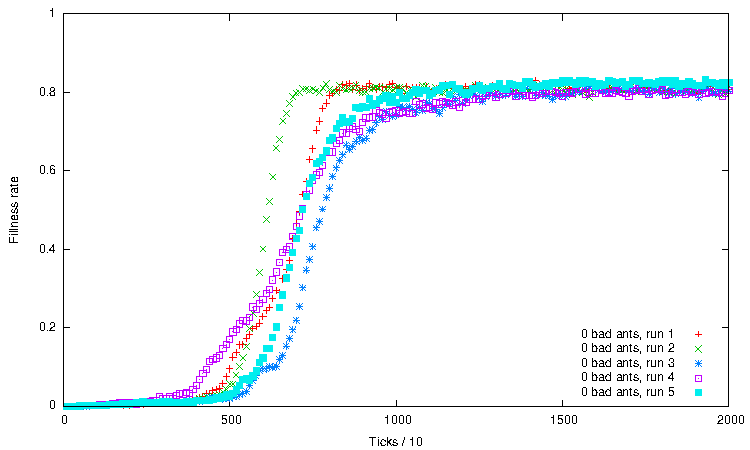
\includegraphics[width=6cm]{images/graph0.pdf}
  \end{minipage}
  \begin{minipage}[b]{0.5\linewidth}
    \centering
    \caption{0 bad ants, one breed }\label{fig:images/graph0oneBreed}
    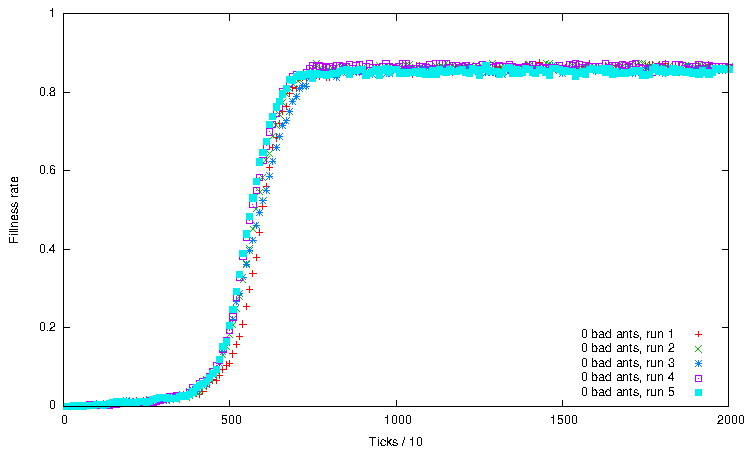
\includegraphics[width=6cm]{images/graph0oneBreed.pdf}
  \end{minipage}
  
  \hspace{0.5cm}
  
  \begin{minipage}[b]{0.5\linewidth}
    \centering
    \caption{10 bad ants }\label{fig:images/graph10}
    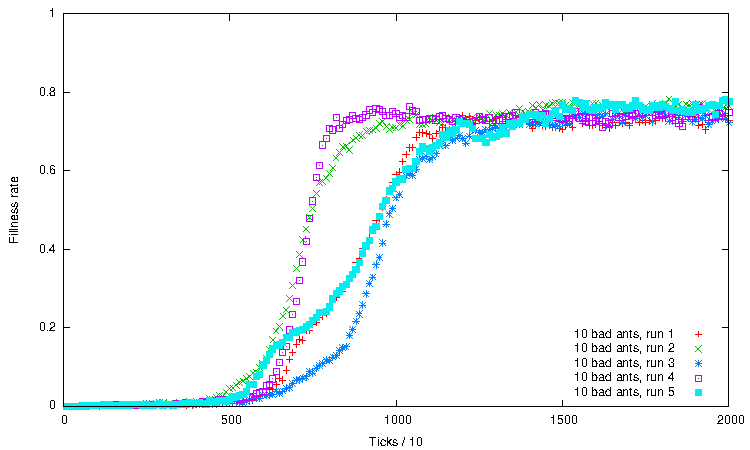
\includegraphics[width=6cm]{images/graph10.pdf}
  \end{minipage}
  \begin{minipage}[b]{0.5\linewidth}
    \centering
    \caption{10 bad ants, one breed }\label{fig:images/graph10oneBreed}
    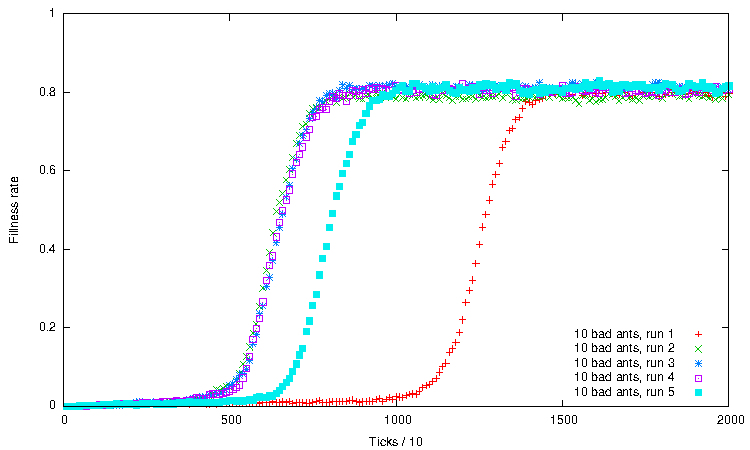
\includegraphics[width=6cm]{images/graph10oneBreed.pdf}
  \end{minipage}
  
  \hspace{0.5cm}

  \begin{minipage}[b]{0.5\linewidth}
    \centering
    \caption{20 bad ants }\label{fig:images/graph20}
    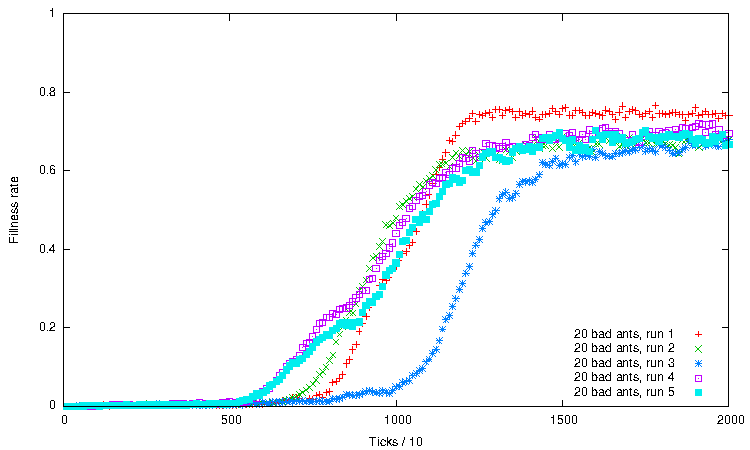
\includegraphics[width=6cm]{images/graph20.pdf}
  \end{minipage}
  \begin{minipage}[b]{0.5\linewidth}
    \centering
    \caption{20 bad ants, one breed }\label{fig:images/graph20oneBreed}
    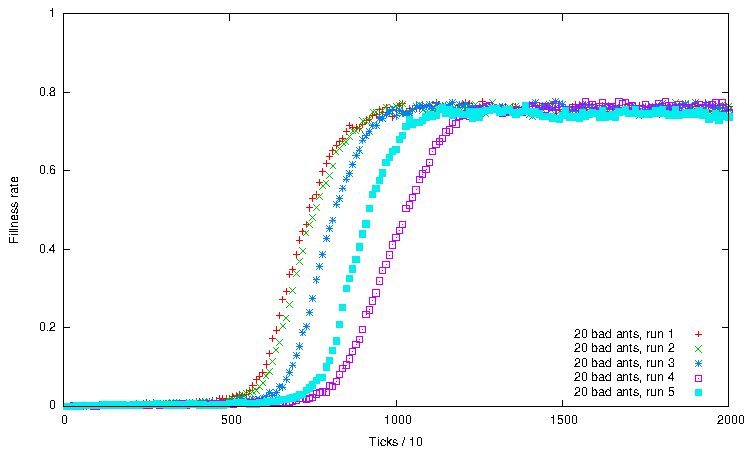
\includegraphics[width=6cm]{images/graph20oneBreed.pdf}
  \end{minipage}
  
  \hspace{0.5cm}

  \begin{minipage}[b]{0.5\linewidth}
    \centering
    \caption{30 bad ants }\label{fig:images/graph30}
    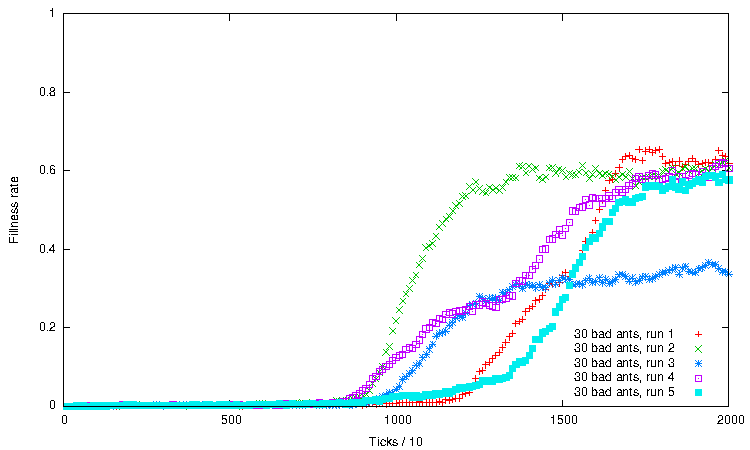
\includegraphics[width=6cm]{images/graph30.pdf}
  \end{minipage}
  \begin{minipage}[b]{0.5\linewidth}
    \centering
    \caption{30 bad ants, one breed }\label{fig:images/graph30oneBreed}
    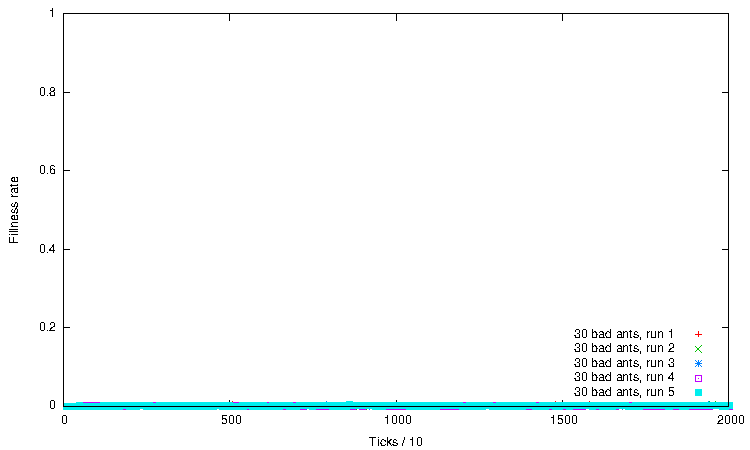
\includegraphics[width=6cm]{images/graph30oneBreed.pdf}
  \end{minipage}
  
\end{figure}

\begin{figure}

  \begin{minipage}[b]{0.5\linewidth}
    \centering
    \caption{40 bad ants }\label{fig:images/graph40}
    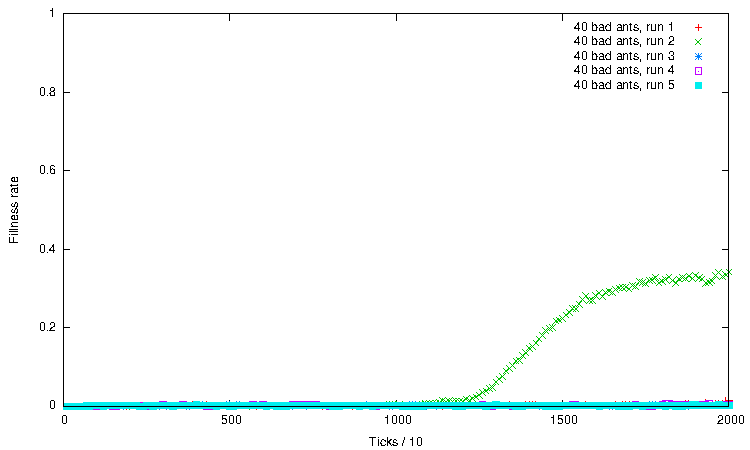
\includegraphics[width=6cm]{images/graph40.pdf}
  \end{minipage}
  \begin{minipage}[b]{0.5\linewidth}
    \centering
    \caption{40 bad ants, one breed }\label{fig:images/graph40oneBreed}
    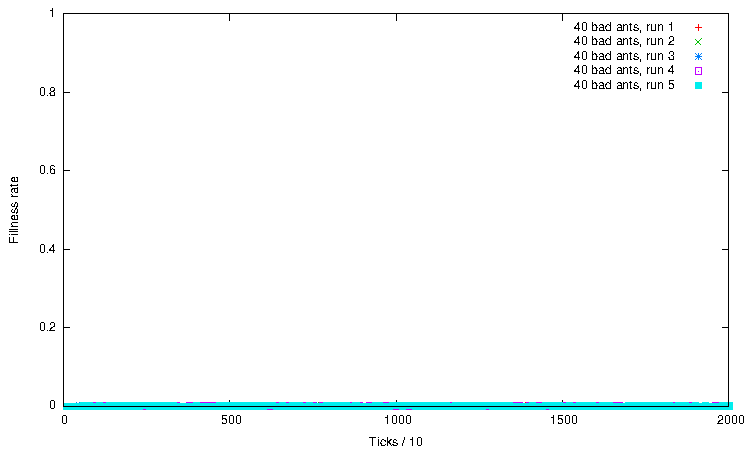
\includegraphics[width=6cm]{images/graph40oneBreed.pdf}
  \end{minipage}
  
  \hspace{0.5cm}
  
  \begin{minipage}[b]{0.5\linewidth}
    \centering
    \caption{50 bad ants }\label{fig:images/graph50}
    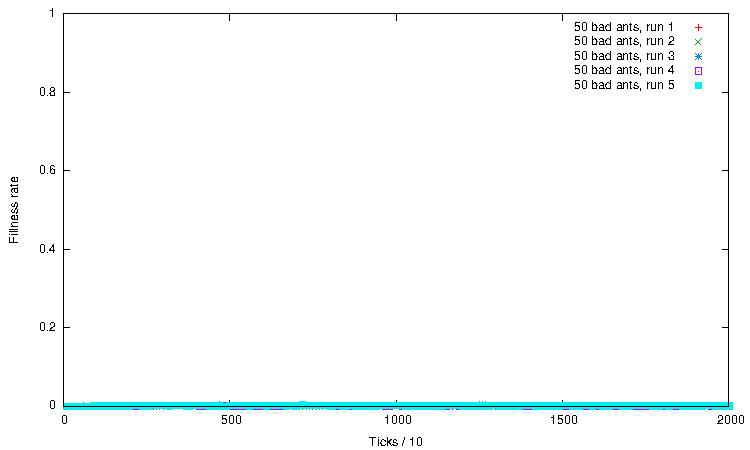
\includegraphics[width=6cm]{images/graph50.pdf}
  \end{minipage}
  \begin{minipage}[b]{0.5\linewidth}
    \centering
    \caption{50 bad ants, one breed }\label{fig:images/graph50oneBreed}
    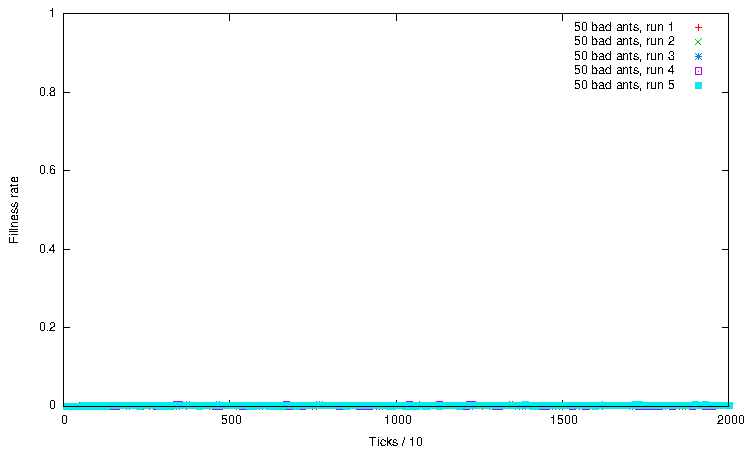
\includegraphics[width=6cm]{images/graph50oneBreed.pdf}
  \end{minipage}
\end{figure}
                    
\section{Applikationsområden}
% Diskutera de frågor som nämns ovan och försöka att sätta in
% laborationen i ett större sammanhang. Kan du se några
% applikationsområden för den här typen av algoritmer? Kan modellen
% utökas för att göras mer intressant?

Tänkta applikationer för denna typen av algoritmer kan vara till
exempel olika mediciner och behandlingar på nano-nivå där mycket enkla
små agenter gemensamt kan konvergera till en komplex behandlingsform.

Kluster av billiga datorer kan jobba gemensamt för att bilda ett
komplext beteende. Distribuerad bearbetning och lagring av data på
datorer runt om världen. Exempel på sådana projekt är exempel
lösningar som räknar fram stora primtal eller behandlar signaler och
letar efter tecken på utomjordiskt liv.

\section{Lösningens begränsningar}
Om ett densitetsreglage fanns till varje färg hade vi problem med att
verkligen få rätt densitet till varje färg. När den första färgen har
slumpats ut vill vi slumpa ut nästa färg. Här misslyckades vi med att
lägga den nya färgen på enbart lediga rutor och alltså kunde vi måla
över den gamla färgen. Detta löste vi genom att ha ett reglage med
densitet och för varje slumpad plats målas med sannolikheten 0.5 den
gröna färgen och med sannolikheten 0.5 den gula färgen. Att ha ett
reglage till varje färg är abolut önskvärt för testning och detta
skulle vara en bra grej att fixa om mer tid fanns.

Vi försökte få in en ticks räknare utan att resultatet blev att en
myra i taget rörde sig. Detta lyckades vi inte med eftersom de metoder
en myra kör förflyttar myran långa sträckor i samma metod. Vi antar
dock att resultaten blir intressant ändå i och med att en myra bara
kollar på pinnar och inte på andra myrors rörelse % TODO (STÄMMET
                                                  % DETTA?  ?

\newpage
\appendix
\pagenumbering{roman}
\section{Källkod}\label{sec:kallkod}
% Källkoden ska finnas tillgänglig i er hemkatalog
% ~/edu/apjava/lab1/. Bifoga även utskriven källkod.
Härefter följer utskrifter från källkoden och andra filer som hör till
denna laboration

\subsection{Termites.nlogo}\label{Termites.nlogo}
\begin{footnotesize}
  \verbatiminput{../src/Termites.nlogo}
\end{footnotesize}
\end{document}
